% MANUSCRIPT STATUS: DIGITAL_RESULTS_AVAILABLE
% Evidence: SYNTHETIC_SIM. NTN is not always better. Not operator KPIs.
\documentclass[11pt]{article}
\usepackage[margin=1in]{geometry}
\usepackage{booktabs,hyperref}
\title{Decision Boundaries for Terrestrial, Edge, Peer, Offline, and NTN Fallback Under Compound Service Disruptions}
\author{Edmund Gunn Jr.\\Independent researcher --- no University of Oulu affiliation claimed}
\date{\today}
\begin{document}
\maketitle
\begin{center}\textbf{RESULT BANNER.} Simulation sweeps only. NTN fallback is not universally superior. Not SUBMITTED.\end{center}
\begin{abstract}
Paper~III compares terrestrial-baseline, static-NTN, fallback, and adaptive policies under seeded outage and compound power+radio failures~\cite{3gpp_tr38821}. Delay/capacity values are documented assumptions, not campaign measurements. Edge I/O device measurement remains \texttt{PHYSICAL\_PENDING}.
\end{abstract}
\section{Introduction}
\label{sec:intro}
Non-terrestrial access can restore a path when terrestrial radio fails, or it can add delay and capacity shortfalls that push a session below its minimum-useful operating point~\cite{3gpp_tr38821,3gpp_ts22261,itur_m2160}.
Paper~III therefore treats NTN as one path among terrestrial, offline, and (named, not separately simulated here) edge/peer alternatives.
The hypothesis to reject is ``NTN always improves min-useful service versus a terrestrial baseline.''

The runnable engine is \texttt{src/ntn\_resilience/experiment.py} with policies \texttt{terrestrial\_baseline}, \texttt{static\_ntn}, \texttt{fallback}, and \texttt{adaptive}.
Sweeps cover NTN latency, capacity, and visibility; a compound power+radio failure; a configured GEO RTT contrast; and a below-min capacity probe.
Nothing in this manuscript is an operator KPI or a field satellite measurement.

\section{Method}
Pre-registered experiment \texttt{rq3\_gary\_failover\_sweeps}: seeds 1,2,7,42; policies terrestrial\_baseline, static\_ntn, fallback, adaptive; compound power outage; sweeps over NTN latency, capacity, visibility.
Delay class \texttt{leo\_tr38821} is literature-backed, not measured.
Edge I/O contributes measurement contracts only; IMU is not absolute pose.

\section{Results}
\label{sec:results}
Generated from \texttt{results/experiments/rq3\_gary\_failover\_sweeps.json} by \texttt{paper/scripts/generate\_tables.py}.
Missing file $\Rightarrow$ \texttt{RESULT\_PENDING}.
A compact extract is \texttt{paper/artifacts/rq3\_experiment\_summary.json}.

\paragraph{When NTN helps.}
Base-case (compound, LEO) mean min-service: terrestrial 0.7396, static/fallback/adaptive 0.8281. On the latency$\times$visibility grid (capacity held at the LEO planning value) every NTN-aware cell beat terrestrial (27 helps, 0 worse, 0 ties). NTN does \emph{not} help when configured GEO RTT 550.0~ms exceeds max-latency 500.0~ms: static\_ntn min-service 0.1302 versus terrestrial 0.7396; fallback equals terrestrial (0.7396). The same pattern appears at NTN capacity 0.5~Mbps $<$ min-capacity 1.0~Mbps: static\_ntn 0.1302 versus terrestrial 0.7396. Hypothesis ``NTN always better'' rejected: true. All numbers are \texttt{SYNTHETIC\_SIM}.

\begin{table}[h]\centering
\caption{RQ3 policy means across seeds (SYNTHETIC\_SIM; not operator KPIs). Recovery column is steps-to-min-service per seed (NA = never recovered).}
\begin{tabular}{lccc}\toprule
policy & mean uptime & mean min-service & recovery steps by seed \\\midrule
terrestrial\_baseline & 0.7396 & 0.7396 & 2,2,4,2 \\
static\_ntn & 0.8281 & 0.8281 & 1,1,3,1 \\
fallback & 0.8281 & 0.8281 & 1,1,3,1 \\
adaptive & 0.8281 & 0.8281 & 1,1,3,1 \\
\bottomrule\end{tabular}\end{table}

\begin{table}[h]\centering
\caption{Decision region: adaptive minus terrestrial min-service (positive = NTN-aware policy helps). SYNTHETIC\_SIM.}
\begin{tabular}{lccc}\toprule
NTN latency (ms) & 0.5 & 0.85 & 0.99 vis. \\\midrule
20 & 0.0469 & 0.0885 & 0.099 \\
40 & 0.0469 & 0.0885 & 0.099 \\
60 & 0.0469 & 0.0885 & 0.099 \\
\bottomrule\end{tabular}\end{table}


Under the compound LEO base case, NTN-aware policies raise mean min-service relative to terrestrial-only (see generated policy table).
On the latency$\times$visibility grid with NTN capacity held at the LEO planning value, every adaptive-minus-terrestrial cell is positive, and the gain grows with visibility (see generated decision table).
Recovery steps to min-service are also shorter for NTN-aware policies than for terrestrial-baseline in this run (seed-wise column of the policy table).

\begin{figure}[h]
\centering
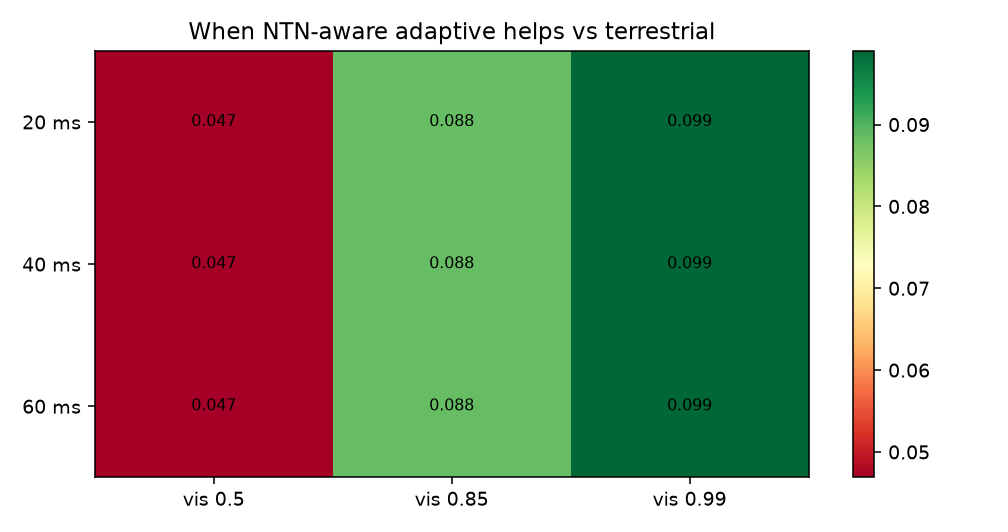
\includegraphics[width=0.95\textwidth]{figures/rq3_adaptive_minus_terrestrial.png}
\caption{Adaptive minus terrestrial min-service on the latency$\times$visibility grid. Positive means the NTN-aware policy helps. SYNTHETIC\_SIM.}
\end{figure}

\begin{figure}[h]
\centering
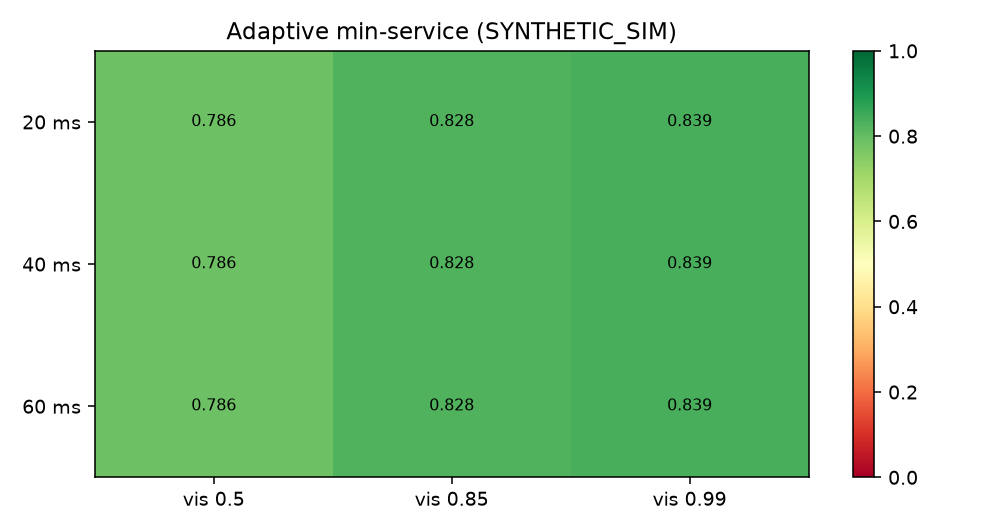
\includegraphics[width=0.95\textwidth]{figures/rq3_adaptive_min_service_heatmap.png}
\caption{Adaptive min-service heatmap (latency $\times$ visibility). SYNTHETIC\_SIM.}
\end{figure}

\paragraph{When NTN does not help.}
\begin{table}[h]\centering
\caption{LEO TR-backed latency versus configured GEO RTT (550~ms). GEO exceeds max\_latency\_ms=500, so NTN can be on-path without meeting min-service.}
\begin{tabular}{lcccc}\toprule
policy & LEO RTT (ms) & LEO min-service & GEO RTT (ms) & GEO min-service \\\midrule
terrestrial\_baseline & 40.0 & 0.7396 & 550.0 & 0.7396 \\
static\_ntn & 40.0 & 0.8281 & 550.0 & 0.1302 \\
fallback & 40.0 & 0.8281 & 550.0 & 0.7396 \\
adaptive & 40.0 & 0.8281 & 550.0 & 0.7396 \\
\bottomrule\end{tabular}\end{table}

\begin{table}[h]\centering
\caption{Capacity probe below min\_capacity\_mbps (SYNTHETIC\_SIM). NTN path may be selected without meeting min-useful service.}
\begin{tabular}{lcccc}\toprule
policy & NTN cap (Mbps) & min cap (Mbps) & mean min-service & below min \\\midrule
terrestrial\_baseline & 0.5 & 1.0 & 0.7396 & True \\
static\_ntn & 0.5 & 1.0 & 0.1302 & True \\
fallback & 0.5 & 1.0 & 0.7396 & True \\
adaptive & 0.5 & 1.0 & 0.7396 & True \\
\bottomrule\end{tabular}\end{table}

\begin{table}[h]\centering
\caption{Compound power+radio failure versus simple radio outage (SYNTHETIC\_SIM).}
\begin{tabular}{lccc}\toprule
policy & simple min-service & compound min-service & delta (compound$-$simple) \\\midrule
terrestrial\_baseline & 0.8854 & 0.7396 & -0.1458 \\
static\_ntn & 0.9896 & 0.8281 & -0.1615 \\
fallback & 0.9896 & 0.8281 & -0.1615 \\
adaptive & 0.9896 & 0.8281 & -0.1615 \\
\bottomrule\end{tabular}\end{table}


Three protocol-declared probes reject ``NTN always better'':
\begin{itemize}
\item Configured GEO RTT $550$~ms exceeds max-latency $500$~ms. \texttt{static\_ntn} then sits on a path that fails min-service; fallback and adaptive collapse to the terrestrial min-service (no gain). Terrestrial-baseline is unchanged, as it never uses NTN.
\item NTN capacity $0.5$~Mbps $<$ min-capacity $1.0$~Mbps. \texttt{static\_ntn} again falls well below terrestrial; fallback/adaptive match terrestrial because they keep the terrestrial path when it is up and cannot meet min-service on the thin NTN path.
\item Compound power+radio versus simple radio: every policy loses min-service under compound failure, and NTN-aware policies lose more than the terrestrial baseline because the engine also blacks out the NTN terminal without power.
\end{itemize}

\begin{figure}[h]
\centering
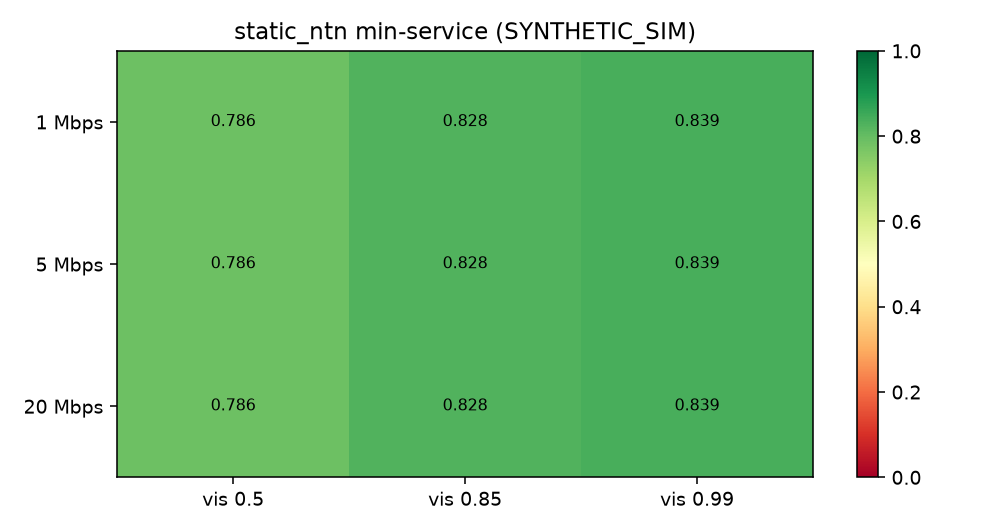
\includegraphics[width=0.95\textwidth]{figures/rq3_static_ntn_capacity_visibility.png}
\caption{\texttt{static\_ntn} min-service on the capacity$\times$visibility grid. Low visibility shrinks the region where staying on NTN preserves min-service. SYNTHETIC\_SIM.}
\end{figure}

CSV companions for all figures live under \texttt{paper/figures/} so the plots can be rebuilt without typing numbers into the PDF.

\section{Limitations}
\label{sec:limitations}
These are seeded simulations under documented assumptions, not operator KPIs, not field NTN, not DEVICE\_MEASURED Edge I/O, and not a University of Oulu affiliation claim~\cite{itur_m2160,3gpp_tr38821}.
GEO RTT is a configured envelope ($550$~ms), not a measured satellite campaign.
Visibility fractions are sensitivity knobs, not orbit-pass statistics.
Edge/peer paths are named in the title for the broader thesis framing; this experiment's action space is terrestrial / NTN / offline.
Independent human reproduction of the digital packet remains PENDING.
\texttt{DIGITAL\_RESULTS\_VALIDATED} means the digital engine reproduced and the help/hurt regions were read from JSON --- not that the paper is submitted or camera-ready.

\bibliographystyle{plain}
\bibliography{bibliography}
\end{document}
